\documentclass{beamer}

\usetheme[numbering=fullbar]{focus} % Use the Focus theme supplied with the template
% Add option [numbering=none] to disable the footer progress bar
% Add option [numbering=fullbar] to show the footer progress bar as always full with a slide count

\newcommand{\R}{\mathbb R}

% Uncomment to enable the ice-blue theme
\definecolor{main}{RGB}{0,0,50}
\definecolor{background}{RGB}{240, 247, 255}

%\usefonttheme{professionalfonts}

\usepackage{tikz}
\usetikzlibrary{calc,decorations.pathmorphing,shapes}

\newcounter{sarrow}
\newcommand\xrsquigarrow[1]{%
\stepcounter{sarrow}%
\mathrel{\begin{tikzpicture}[baseline= {( $ (current bounding box.south) + (0,-0.5ex) $ )}]
\node[inner sep=.5ex] (\thesarrow) {$\scriptstyle #1$};
\path[draw,<-,decorate,
  decoration={zigzag,amplitude=0.7pt,segment length=1.2mm,pre=lineto,pre length=4pt}] 
    (\thesarrow.south east) -- (\thesarrow.south west);
\end{tikzpicture}}%
}

\usepackage{booktabs}
\usepackage{tikz-cd}
\usetikzlibrary{graphs,decorations.pathmorphing,decorations.markings}


\title{\LARGE Finite field library and counting points over finite field}
%\hfill\small $L(s,V,L/K)=\displaystyle\prod_v\det(1-\varphi_wNv^{-s}|V^{I_{w}})^{-1}$}

\subtitle{Computing project -- Part 1}

\author{Jujian Zhang, Yuan Yang and Diego Chicharro}

\institute{LSGNT}

%\titlegraphic{\includegraphics[scale=.3]{image}}

\date{9 December 2021}

\def\arraystretch{1.5}

\begin{document}

\begin{frame}
    \maketitle
\end{frame}

\begin{frame}{Abstract}
    In the first part of our project, we built finite field library, by finding all irreducible polynomials 
    of degree $n$ over the prime field $\mathbb{F}_{p}$, and then we
    compute the number of points of a given finite field $\mathbb{F}_{p^n}$ and a given elliptic curve
    $y^2=x^3+ax+b$. 
\end{frame}

\begin{frame}{Define \emph{modp} element}
    First we defined the class \emph{modp} element in Python
    \begin{center}
        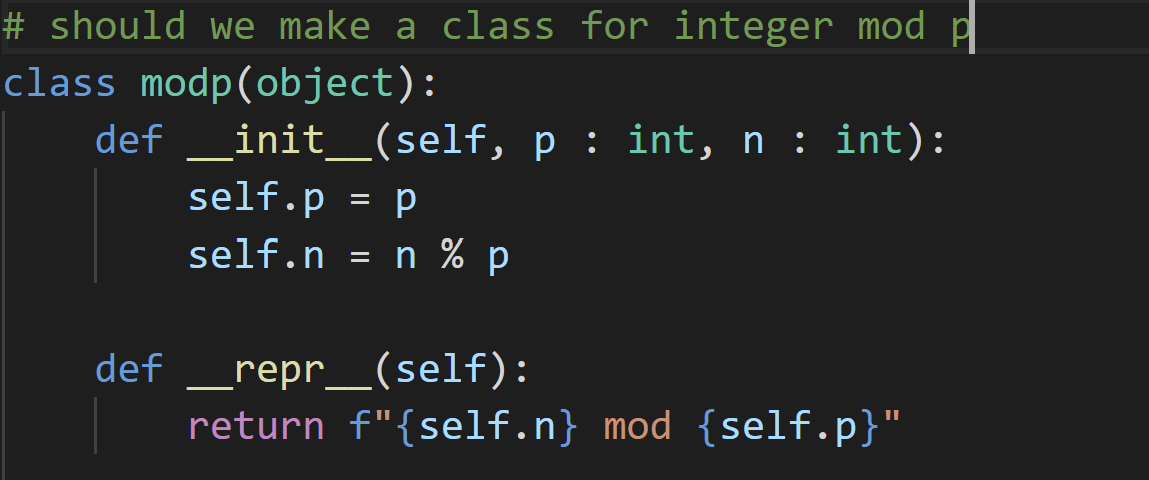
\includegraphics[scale = .4]{modp.png}
    \end{center}
    And operations(+,-,*,/) between them.
    \begin{center}
        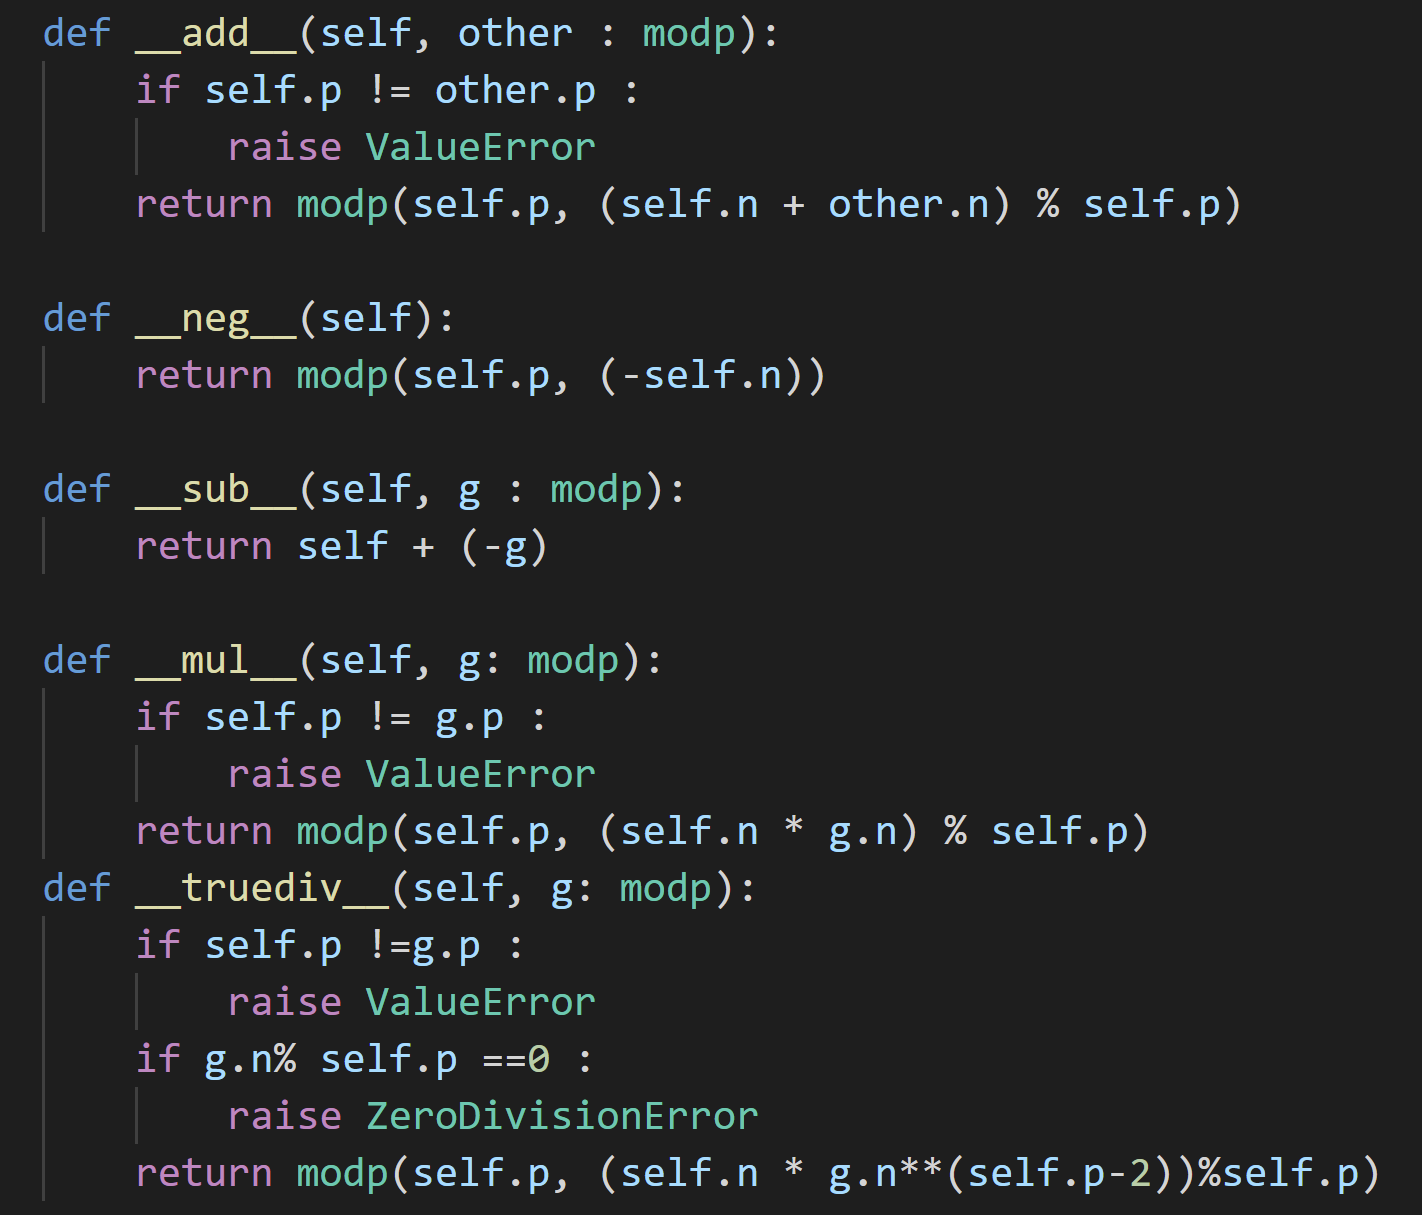
\includegraphics[scale = .4]{modpoperations.png}
    \end{center}
\end{frame}

\begin{frame}{Caution: need to define what is 'equal'!}
    We need to compare if two modp elements are equal.
    \begin{center}
        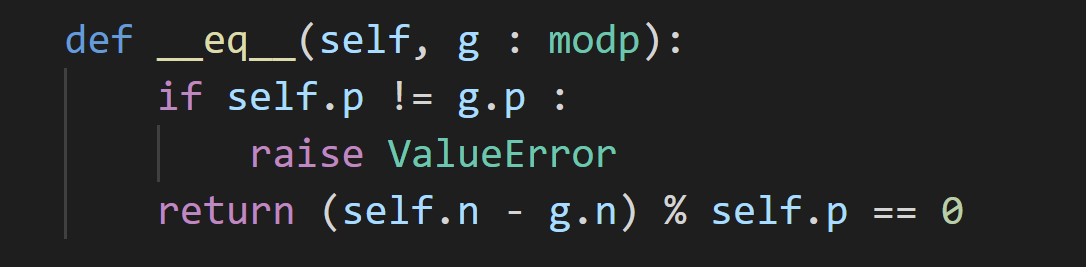
\includegraphics[scale = .5]{modpequal.png}
    \end{center}
\end{frame}

\begin{frame}{Define \emph{modp polynomials}.}
    Then we can define polynomials with modp element coefficients,
    it contains degree, and a coefficients dictionary.
    \begin{center}
        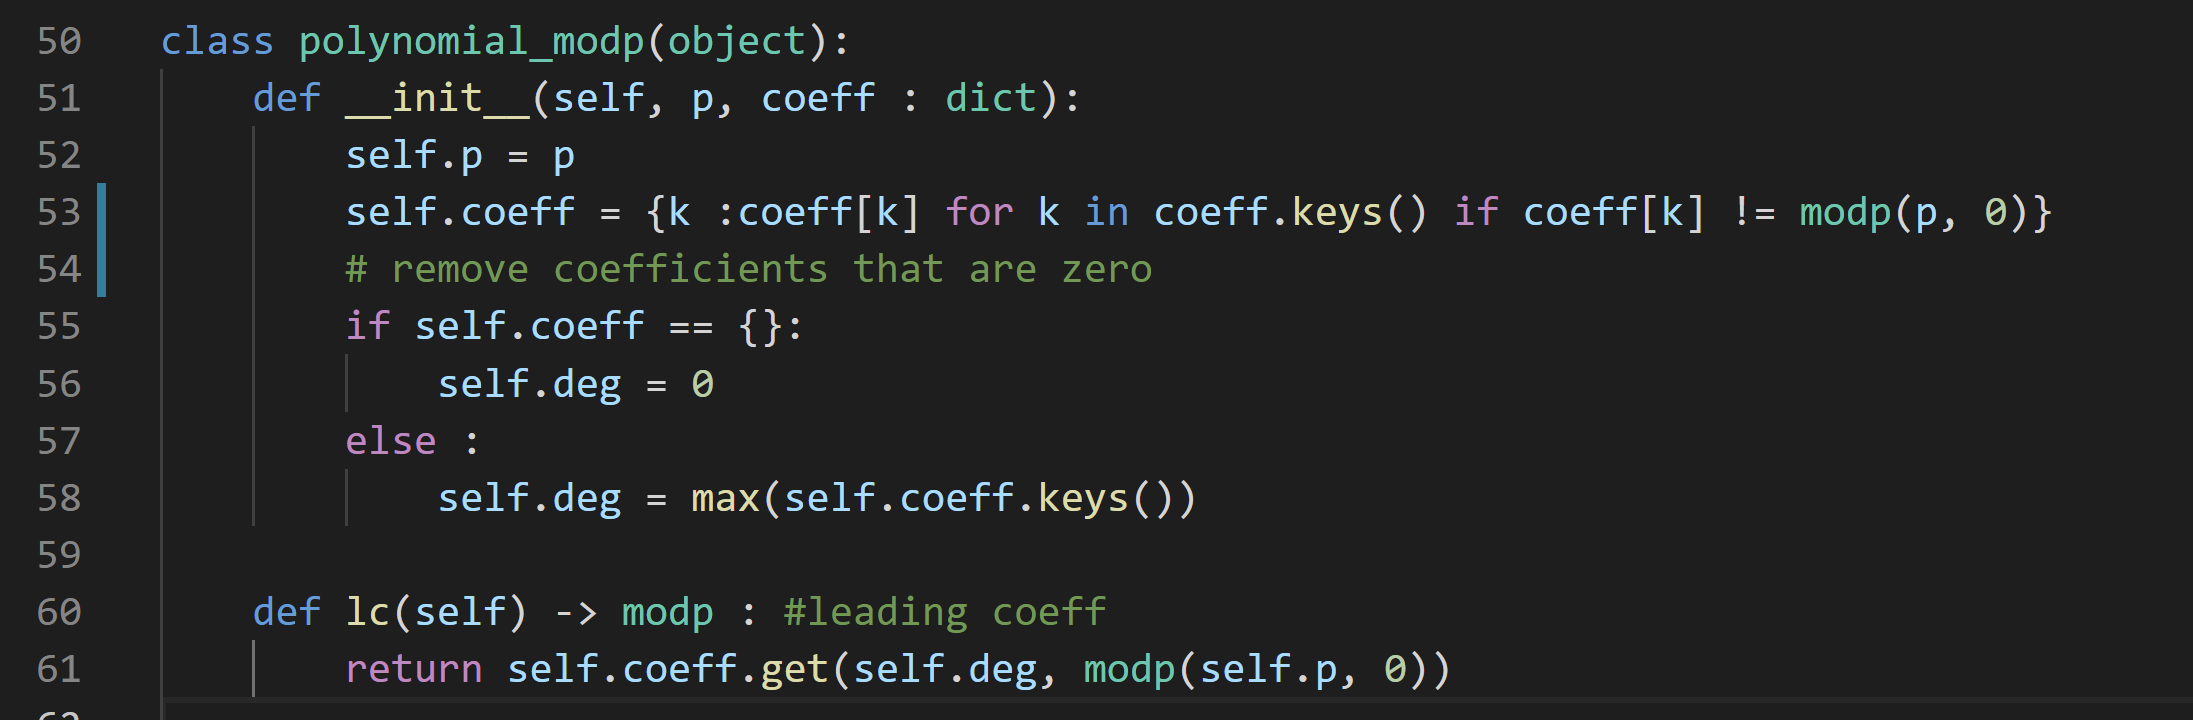
\includegraphics[scale = .5]{modppoly.png}
    \end{center} 
    Notice that we removed all zero coefficient, and we keep the leading coefficient. 
\end{frame}

\begin{frame}{Again, define basic operations between modp polynomials}
    Again, we define (+,-,*) operations between modp polynomials.
    \begin{center}
        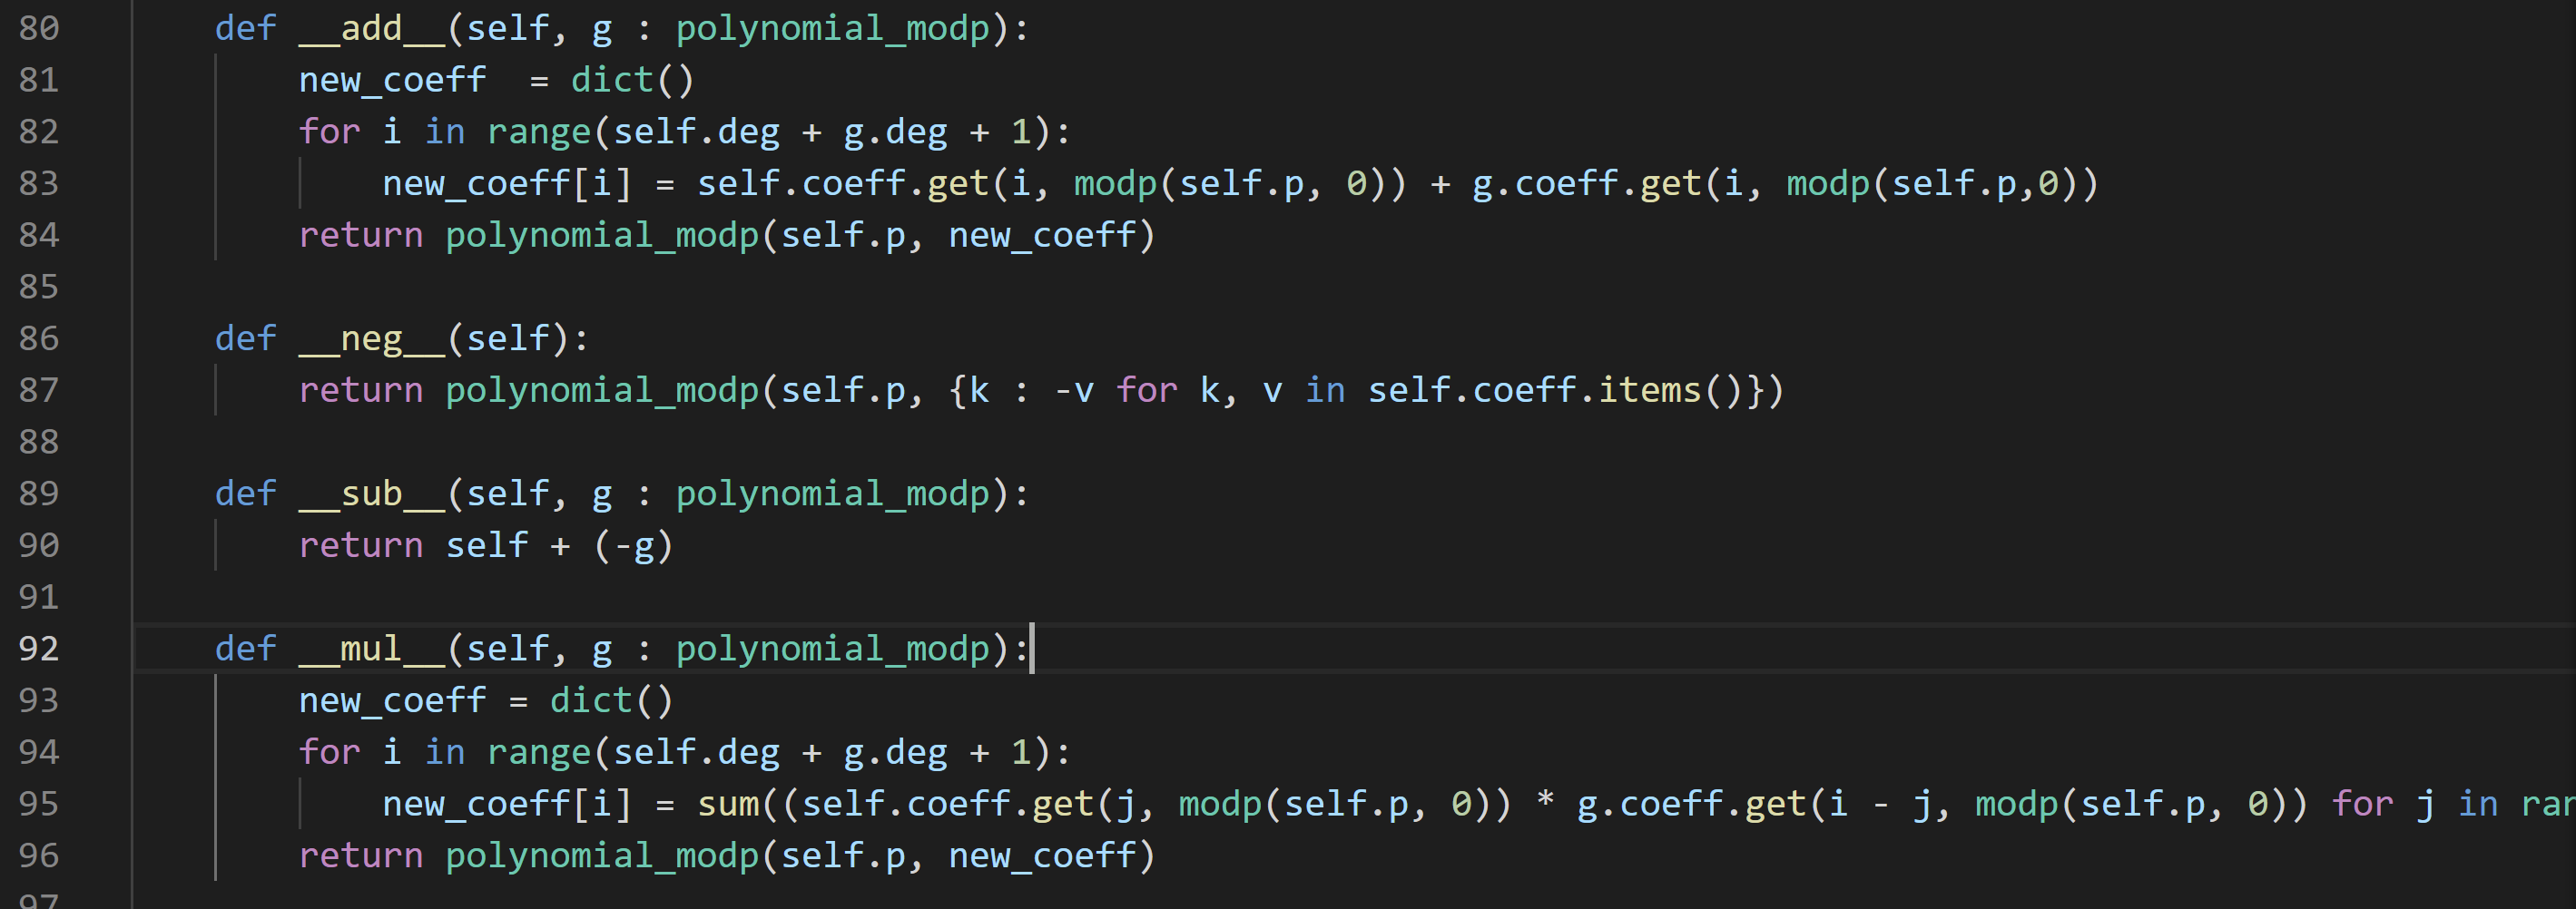
\includegraphics[scale = .5]{polyoperation.png}
    \end{center}
\end{frame}

\begin{frame}{floor division and modulo operation}
    We need floor division.
    \begin{center}
        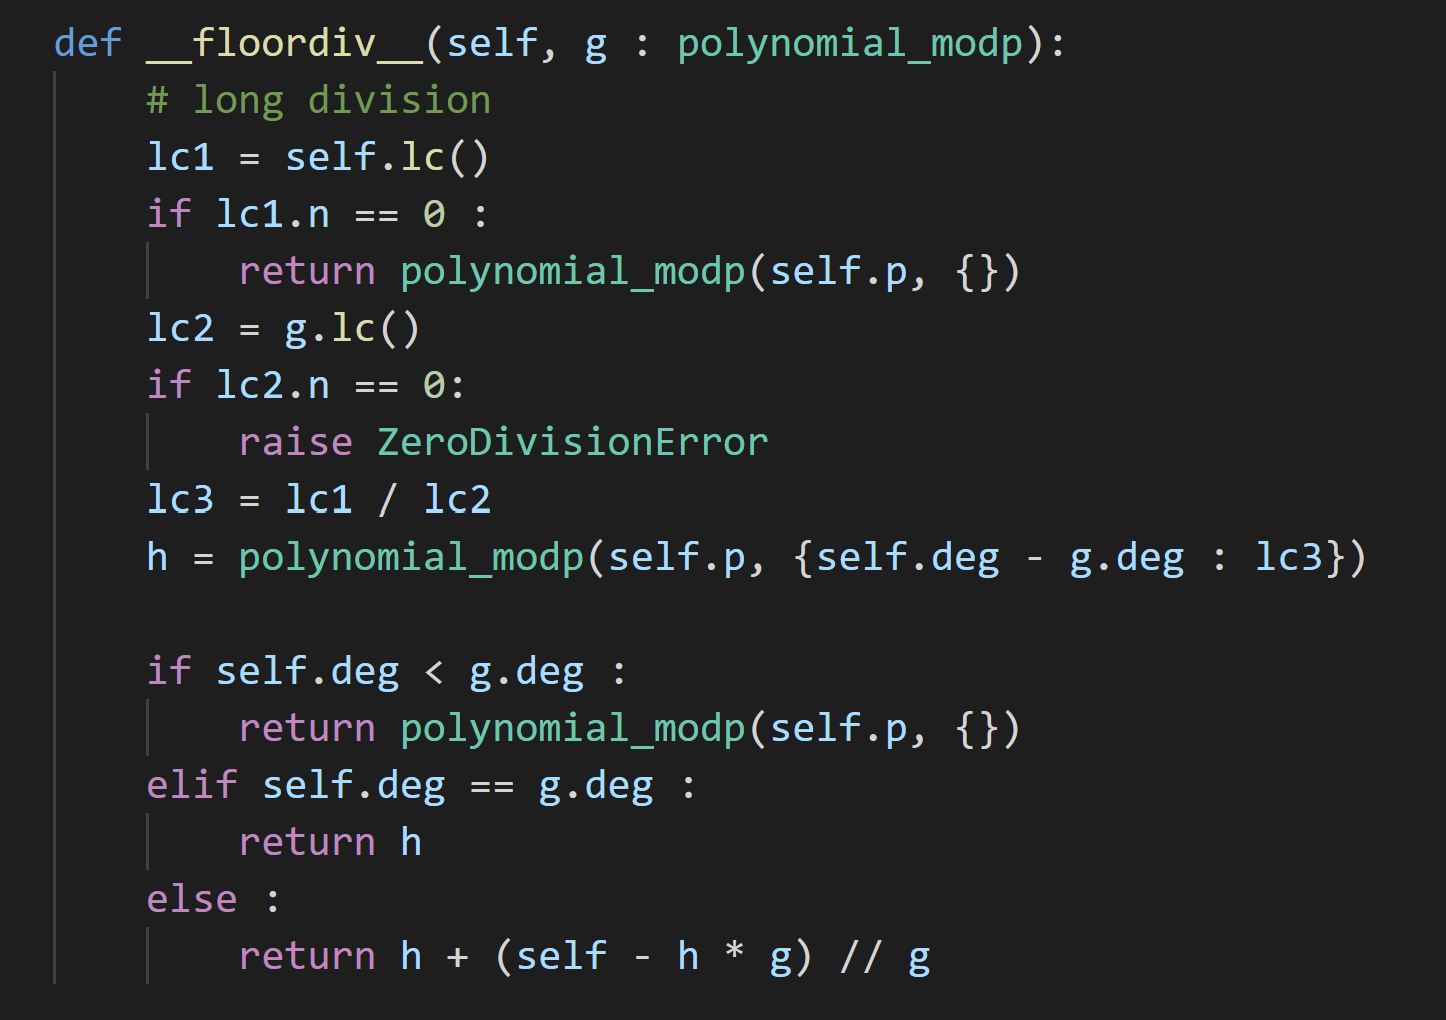
\includegraphics[scale = .5]{floor.png}
    \end{center}
    And the residue polynomial.
    \begin{center}
        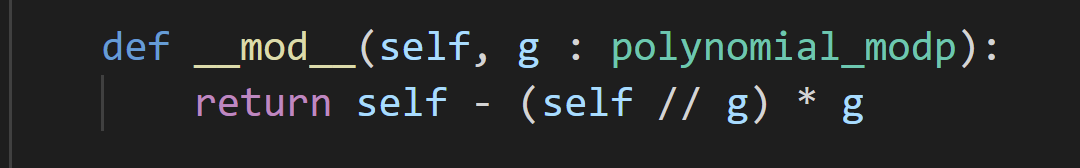
\includegraphics[scale = .5]{module.png}
    \end{center}
\end{frame}

\begin{frame}{Define two \emph{list}s of polynomials!}
    Define all polynomials of degree no more than $n$
    \begin{center}
        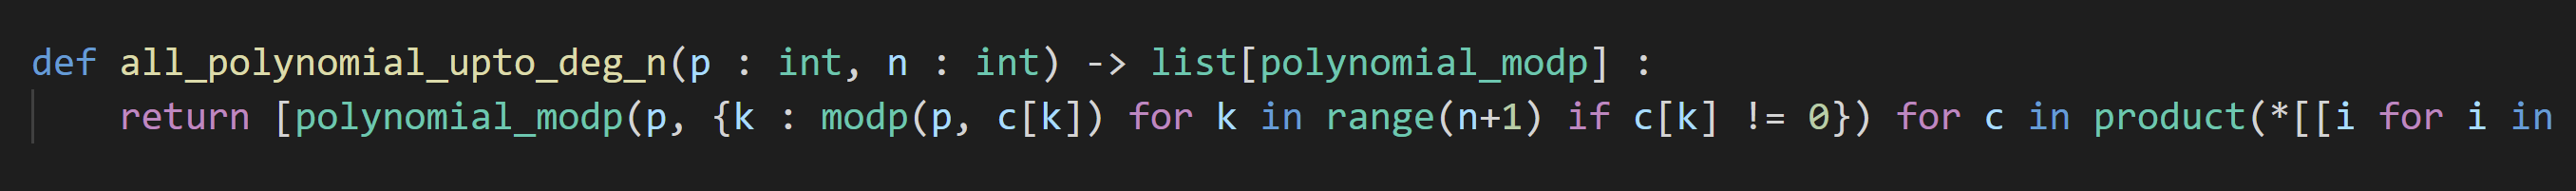
\includegraphics[scale = .5]{allpoly.png}
    \end{center}
    Define all \emph{monic} polynomials of degree no more than $n$
    \begin{center}
        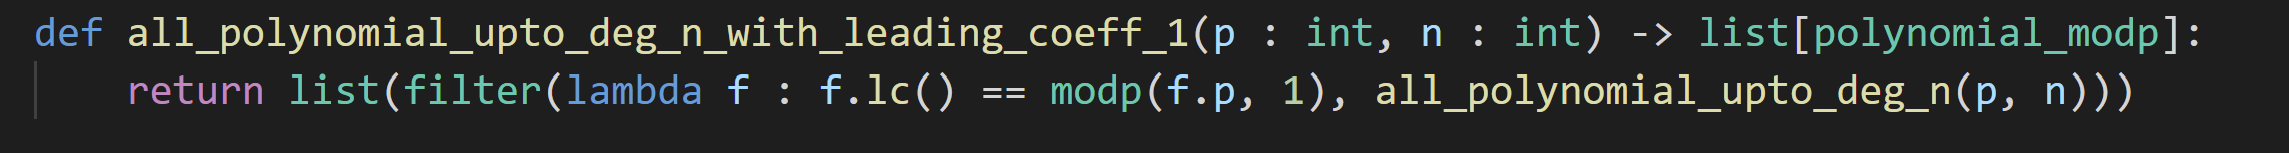
\includegraphics[scale = .5]{allmonicpoly.png}
    \end{center}
\end{frame}

\begin{frame}{Check if a polynomial is composite or irreducible!}
    Define two functions to check if it is composite or irreducible.
    \begin{center}
        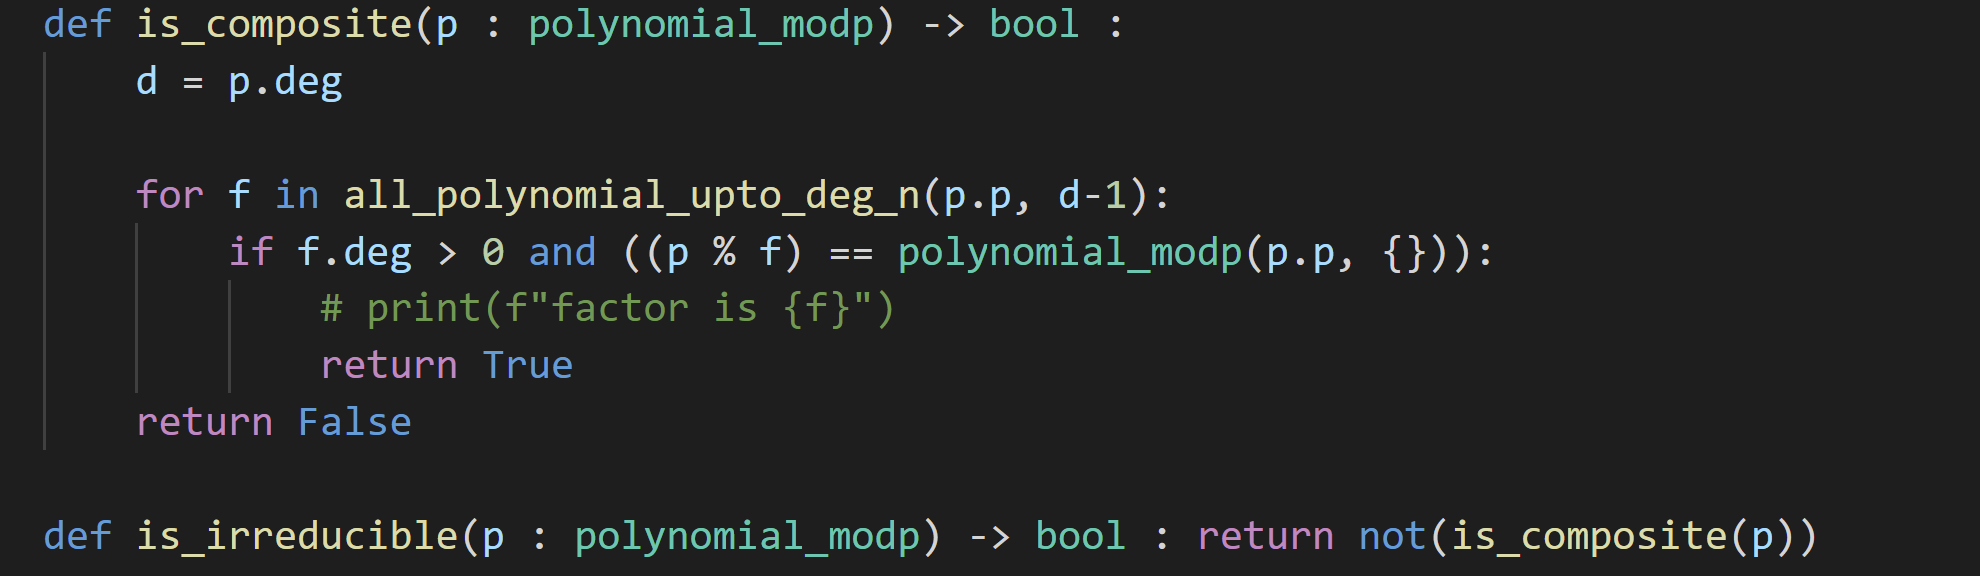
\includegraphics[]{isirre.png}
    \end{center}
\end{frame}

\begin{frame}{Generate all irreducible polynomial of degree no more than $n$}
    \begin{center}
        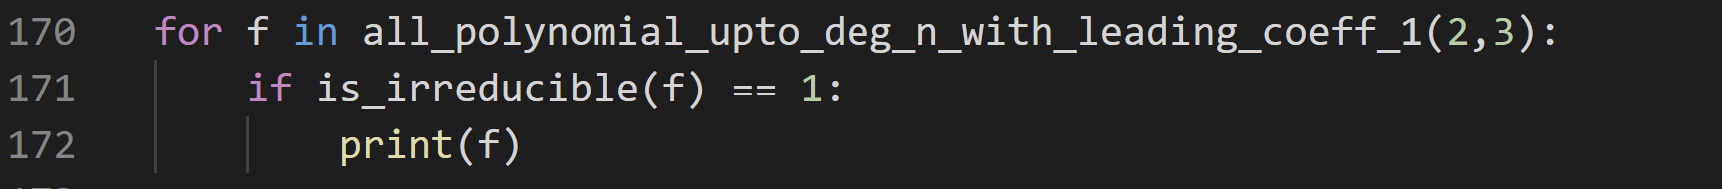
\includegraphics[scale = .5]{allirre.png}
    \end{center}
    \begin{center}
        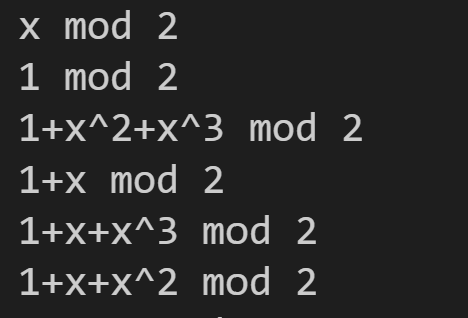
\includegraphics[]{allirreresult.png}
    \end{center}
\end{frame}

\begin{frame}{Generate an irreducible polynomial of degree $n$}
    Find an irreducible polynomial.
    \begin{center}
        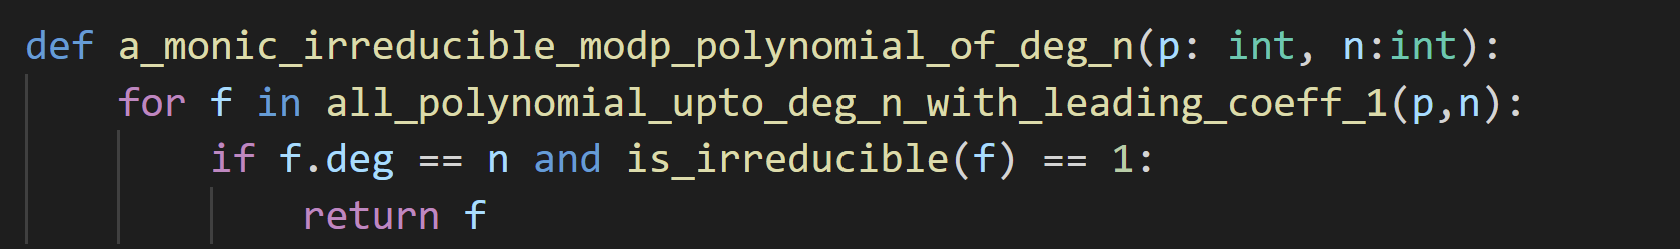
\includegraphics[scale = .5]{generate.png}
    \end{center}
    Have a test!
    \begin{center}
        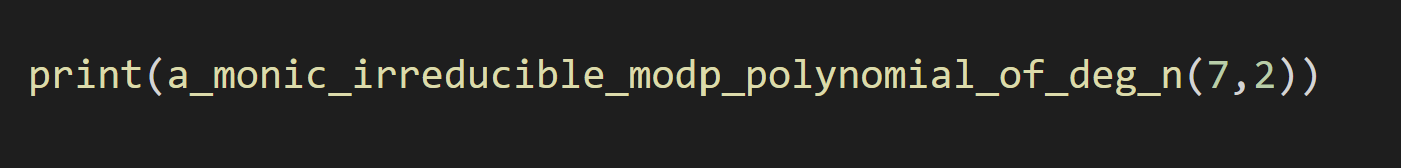
\includegraphics[scale = .5]{testpoly.png}
    \end{center}
    \begin{center}
        
\includegraphics[scale = .5]{testresult1.png}
    \end{center}
\end{frame}

\begin{frame}{Application: Counting points on a given elliptic cueve}
    Given a prime number $p$, degree $n$, coefficients $a,b$, we count the number of
    $\mathbb{F}_{p^n}$ points of the elliptic curve $y^2 = x^3 + ax + b$.
    \begin{center}
        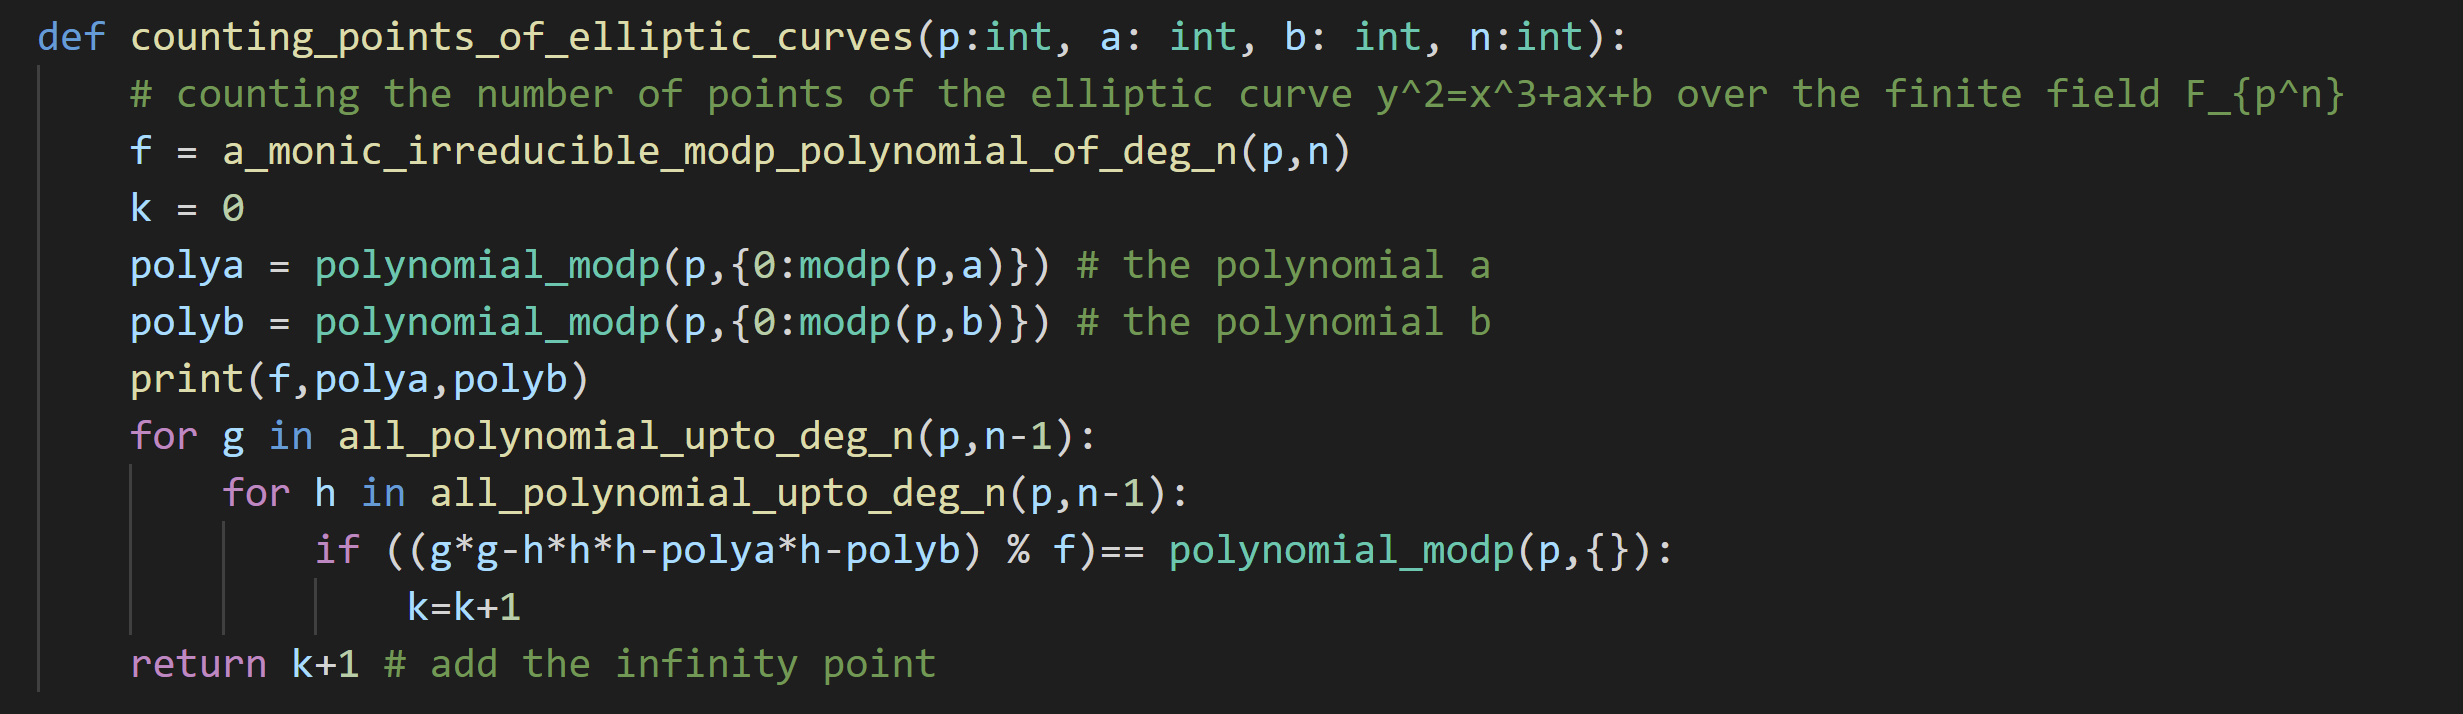
\includegraphics[scale = .5]{count.png}
    \end{center}
    Test!
    \begin{center}
        
\includegraphics[scale = .5]{countelliptic.png}
    \end{center}
    \begin{center}
        
\includegraphics[scale = .5]{elliptictestresult.png}
    \end{center}

\end{frame}

\begin{frame}
    \huge{Thank you!}
\end{frame}

\end{document}


